\section{Implementing the editor calculus}

The implementation of the editor calculus requires

\begin{itemize}
\item implementing the semantics of the calculus and allowing for an
  appropriate visualization of editing
\item implementing a type checker based on the type system
\end{itemize}

but perhaps surprisingly, it involves finding a way to script editor
calculus expressions. In this section we outline this.

\subsection{Implementing the editor calculus semantics}

We model the formation rules of the editor calculus by a collection of
algebraic datatypes. As an example, expressions are given by the
datatype

\begin{lstlisting}[language=elm,%
                   label={aep-without-holes-definition},%
                   gobble=4,%
                   caption={Formation rules (\ref{aep-formation-rules}) modeled in Elm},%
                   ]
    type Aep
        = Eval
        | Sub Aam
        | Child Ast.Child
        | Parent
\end{lstlisting}

The rest of the formation rules are defined similarly.

\subsection{Abstract syntax trees}

Since an AST is a tree data structure, there are a multitude of ways we could
visualize them, and we had to pick a number of representations among many. We
are interested in visualizing the AST to make the editor intuitive for a user.
We are not necessarily interested in finding the ``best'' visualization, nor in
implementing a vast number of different representations.

A very simple representation would be to represent the AST in a textual form,
as seen in figure \ref{fig:ast-in-text-form}.

\begin{figure}[H]
    \Large
    \begin{equation*}
      \cursor{(\app{\breakpoint{(\lambda{x}{(\app{x}{x})})}}
      {(\lambda{x}{(\app{x}{x})})})}
    \end{equation*}
    \caption{An AST visualized in textual form.}
    \label{fig:ast-in-text-form}
\end{figure}

The notation used for this representation follows the notation used by Godiksen
et al.~\pepm. We implemented this representation, as it was straightforward to
implement, and it can provide the user with a compact and formal visualization
of the AST. However, this approach comes with some drawbacks. It can be
difficult to reason about, especially as an AST grows large.

Because of this, we decided to implement another representation in addition to
the textual form. The second approach is by representing it as tree structures
often are, i.e. where nodes are rectangles and branches are lines that grow
downwards, as seen in figure \ref{fig:ast_visual_tree}. A potential variation
of this structure, could be in the form of a horizontal tree spanning from left
to right

Switching between the two visualizations is meant to be as easy as a click of a
button, which allows the user to choose their preferred representation at any
time.

\begin{figure*}
  \center
  \noindent\begin{minipage}{.45\textwidth}
    \center
    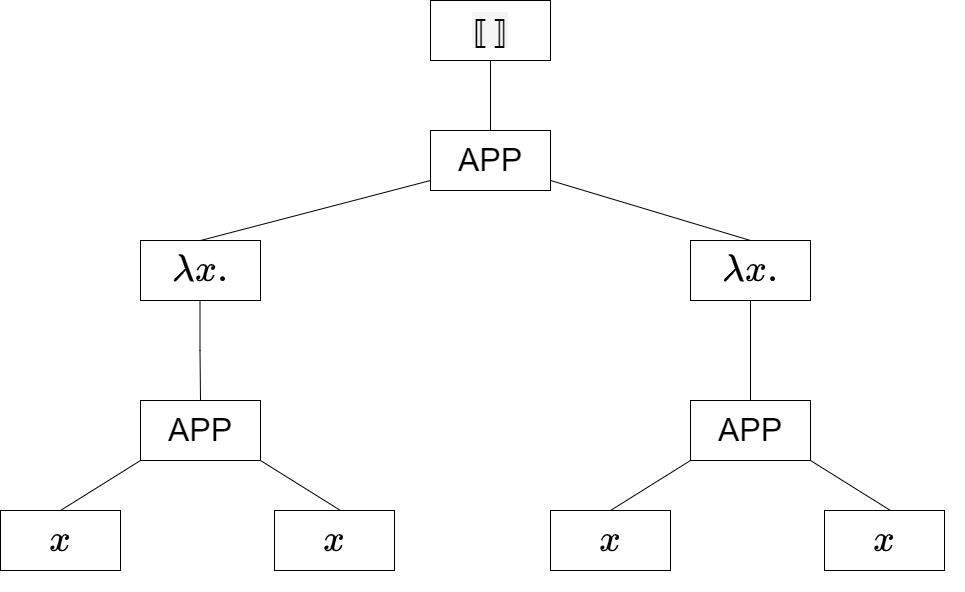
\includegraphics[width=\textwidth]{assets/ast_root_cursor.png}
  \end{minipage}\hfill
  \begin{minipage}{.45\textwidth}
    \center
    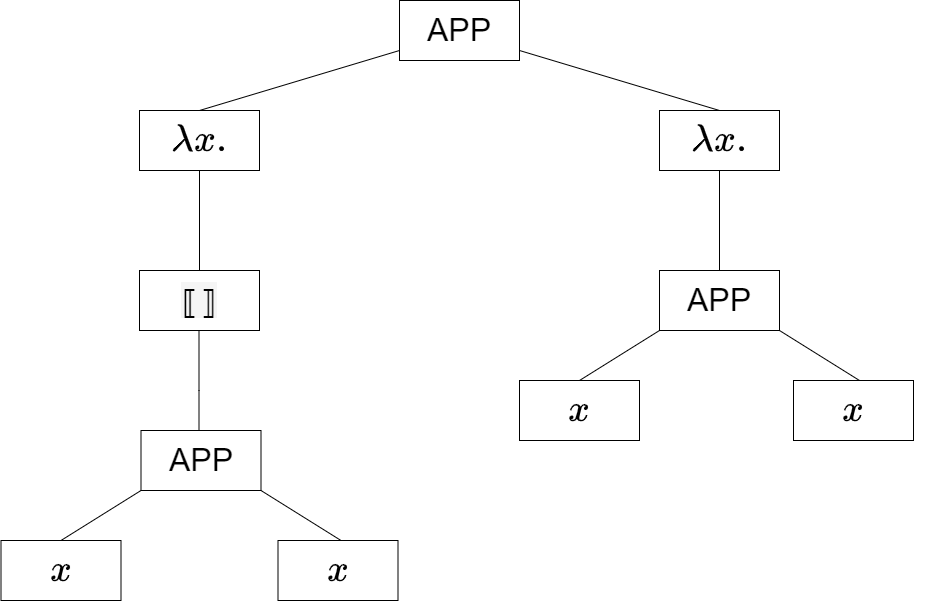
\includegraphics[width=\textwidth]{assets/ast_subtree_cursor.png}
  \end{minipage}\hfill
  \caption{An AST before and after cursor movement visualized in tree form}
  \label{fig:ast_visual_tree}
\end{figure*}

\subsection{Implementing a type checker}

\subsection{Building editor expressions}


%%% Local Variables:
%%% mode: latex
%%% TeX-master: "../pepm2023"
%%% End:
